%%%%%%%%%%%%%%%%%%%%%%%%%%%%%%%%%%%%%%%%%
% Stylish Article
% LaTeX Template
% Version 2.1 (1/10/15)
%
% This template has been downloaded from:
% http://www.LaTeXTemplates.com
%
% Original author:
% Mathias Legrand (legrand.mathias@gmail.com) 
% With extensive modifications by:
% Vel (vel@latextemplates.com)
% Final ACS by:
% Juan Barbosa
% License:
% CC BY-NC-SA 3.0 (http://creativecommons.org/licenses/by-nc-sa/3.0/)
%
%%%%%%%%%%%%%%%%%%%%%%%%%%%%%%%%%%%%%%%%%
\documentclass[fleqn,10pt]{SelfArx}
%\usepackage[superscript]{cite}
\usepackage{wrapfig}
%----------------------------------------------------------------------------------------
%	ARTICLE INFORMATION
%----------------------------------------------------------------------------------------

\JournalInfo{Laboratorio Org\'anica 3, No. 2, 25/08/2017} % Journal information
\Archive{ }

\PaperTitle{Reacci\'on de McMurry} %
%\Keywords{Keyword1 --- Keyword2 --- Keyword3} % Keywords - if you don't want any simply remove all the text between the curly brackets
%\newcommand{\keywordname}{Keywords} % Defines the keywords heading name

%----------------------------------------------------------------------------------------
%	ABSTRACT
%----------------------------------------------------------------------------------------

\Abstract{
\begin{wrapfigure}{r}{0.45\textwidth}
	\centering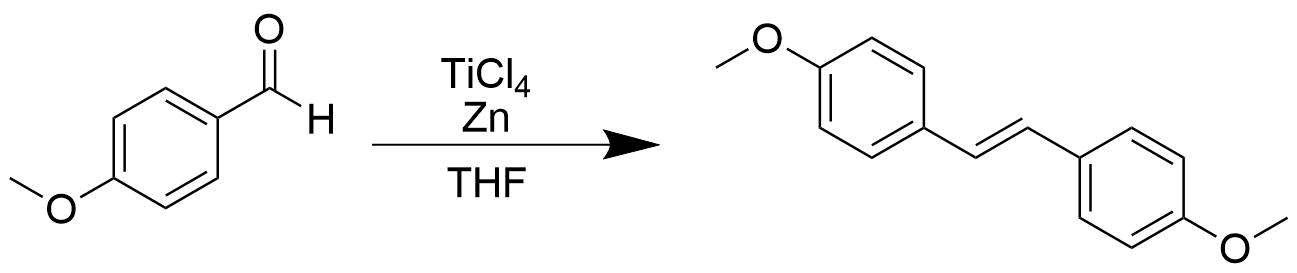
\includegraphics[width=0.9\linewidth]{structures/Reaction.png}
\end{wrapfigure}
}

%----------------------------------------------------------------------------------------

\begin{document}

\flushbottom % Makes all text pages the same height

\maketitle % Print the title and abstract box

%\tableofcontents % Print the contents section

\thispagestyle{empty} % Removes page numbering from the first page



%----------------------------------------------------------------------------------------
%	ARTICLE CONTENTS
%----------------------------------------------------------------------------------------

\section*{Introducci\'on} % The \section*{} command stops section numbering
%------------------------------------------------

La reacci\'on de McMurry fue publicada en 1974, por John E. McMurry. Esta reacci\'on consiste en el acoplamiento carbonilos, para formar alquenos. En este sentido la reacci\'on es an\'aloga al acoplamiento de Sharpless \cite{doi:10.1021/ja00188a068}. Una ventaja de la reacci\'on de McMurry es que es posible realizar acoplamientos intra e inter moleculares de aldeh\'idos y cetonas. Sin embargo el control de la estereoqu\'imica es limitado

La reacci\'on se lleva a cabo usando esp\'ecies de titanio con bajo n\'umero de oxidaci\'on . 

\section{Resultados y Discusi\'on}

El titanio (IV) se reduce en presencia de zinc (\autoref{eq: reduccion}), formando una esp\'ecie divalente oxof\'ilica y reductora \cite{richards2001}. La reacci\'on se lleva a cabo en tetrahidrofurano por dos razones: la primera es que el cloruro de titanio (IV) es soluble en THF, y por otro lado este disolvente no se reduce por las condiciones de la reacci\'on \cite{richards2001}. Esta etapa comprende la primera parte de la reacci\'on, la cual se lleva a cabo a reflujo por una hora.
\begin{equation}\label{eq: reduccion}
	\ce{TiCl_4 + Zn ->[\Delta] TiCl2 + ZnCl2}
\end{equation}

Una vez se adiciona el \textit{p}-metoxibenzaldehido al medio de reacci\'on un electr\'on de valencia del titanio ataca al ox\'igeno generando a su vez un radical sobre el carbono carbon\'ilico (). Posteriormente el radical de titanio ataca de forma an\'aloga a otra mol\'ecula de benzaldehido (). Posteriormente tiene lugar la ciclaci\'on, en este punto dos posibles intermediarios se pueden formar dependiendo de la orientaci\'on de los ciclos. Teniendo en cuenta el volumen de los ciclos y las interacciones desfavorables que se tienen si ambos se encuentran muy cerca, la ciclaci\'on se da a manera de puente, formando un pinacol (). Posteriormente un \'atomo de zinc reduce al titanio y se da la liberaci\'on del \'oxido de titanio (IV), y se genera el producto de estereoqu\'imica \textit{E} \cite{richards2001}.
\begin{scheme}[h]
	\centering
	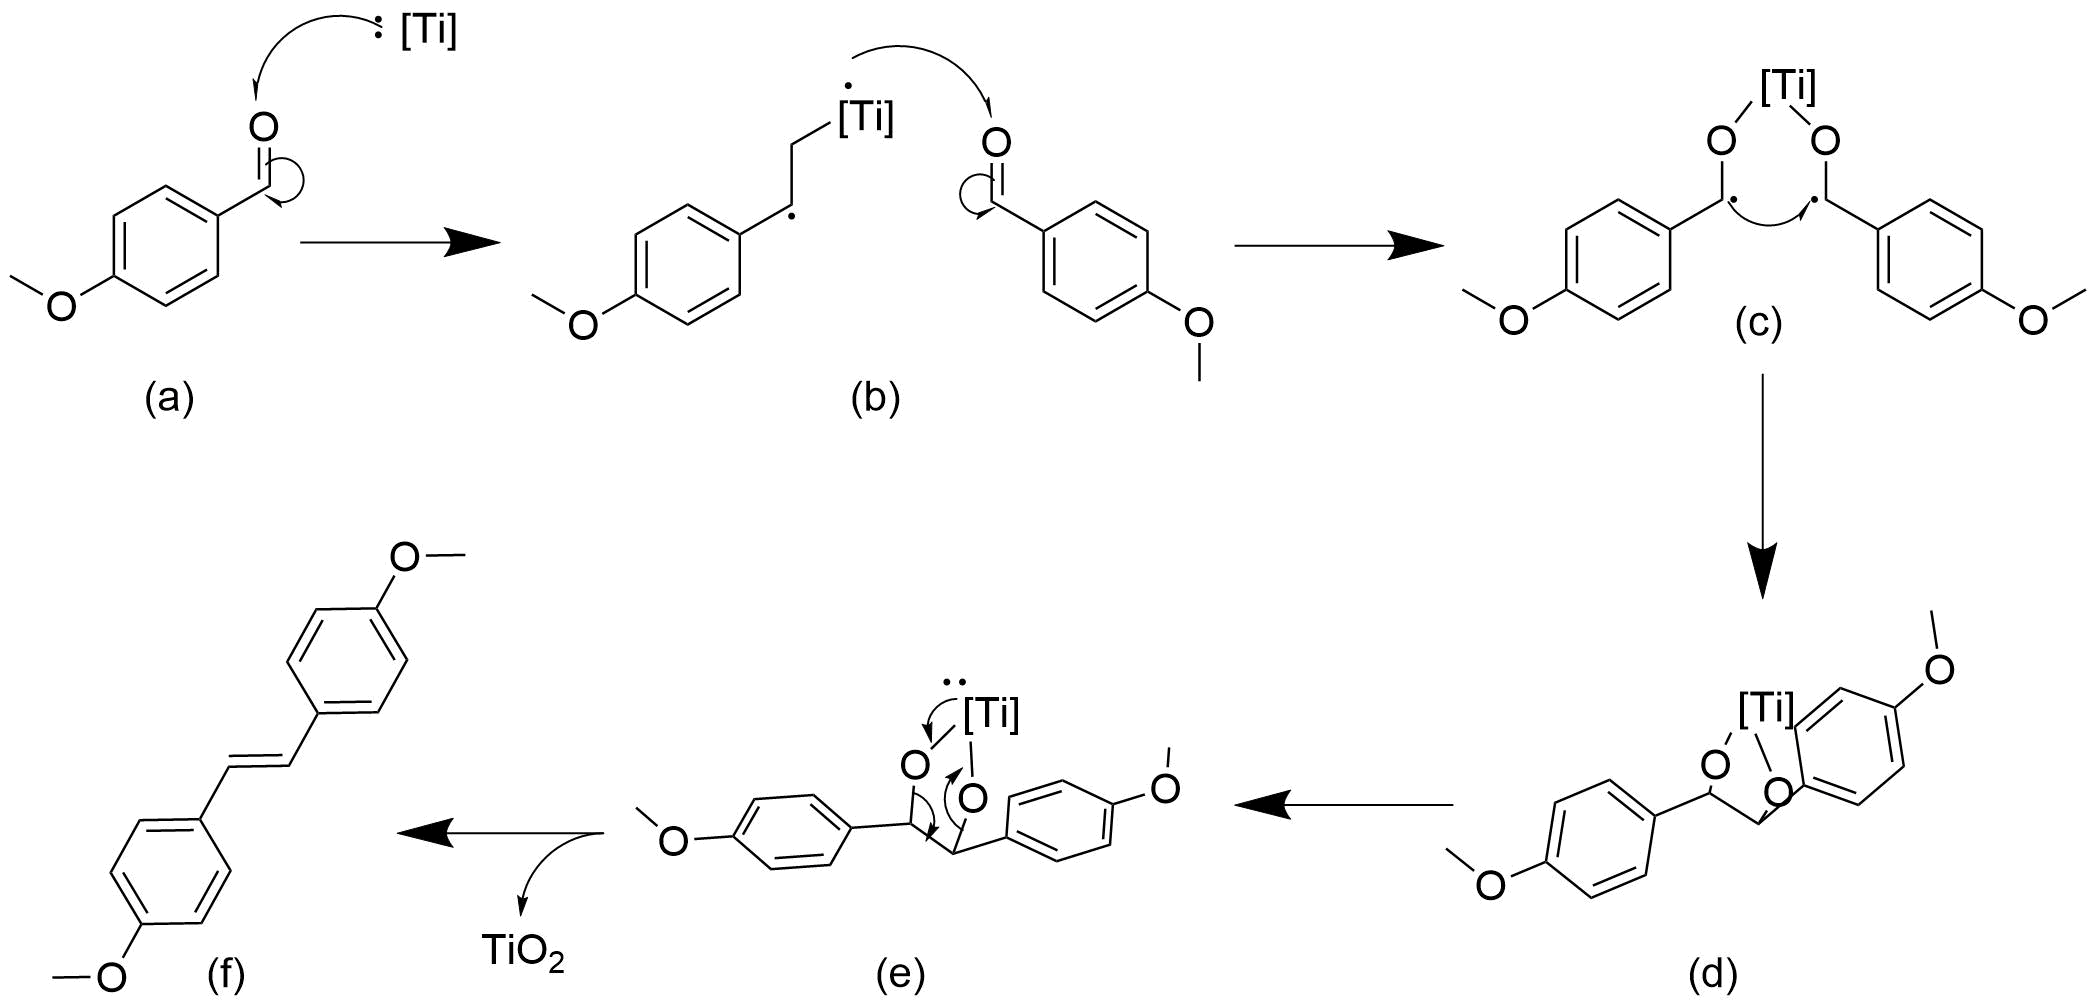
\includegraphics[width = \linewidth]{structures/mechanism.png}
	\caption{Mecanismo de reacci\'on propuesto.}
\end{scheme}

\section{Conclusiones}
\section{Secci\'on experimental}
50 mL de tetrahidrofurano previamente seco por 48 horas usando tamiz molecular, se agregan sobre un bal\'on de dos bocas junto con Zinc (15.0 mmol) y cloruro de titanio (7.5 mmol). La soluci\'on se lleva a reflujo por 1 hora, pasada la cual se adiciona \textit{p}-metoxibenzaldehido (5.0 mmol). La reacci\'on se lleva a cabo a 55 $^\circ$C por 18 horas. La reacci\'on es tratada en 50 mL de \'acido clorh\'idrico 1 M. Se realiza una filtraci\'on en celita y una extracci\'on l\'iquido l\'iquido con dos lavados de 15 mL de diclorometano. El extracto se baña en salmuera y se extrae el sobrenadante, el cual se seca usando sulfato de magnesio y se evapora el disolvente.
%----------------------------------------------------------------------------------------
%	REFERENCE LIST
%----------------------------------------------------------------------------------------
\phantomsection
\bibliography{informe}
\bibliographystyle{unsrt}

%----------------------------------------------------------------------------------------
\newpage
\onecolumn
\section{Informaci\'on suplementaria}\label{sec: complementaria}
\end{document}